\chapter*{Conclusion générale et perspectives} % Ne numérote pas le chapitre
\addcontentsline{toc}{chapter}{Conclusion générale et perspectives} % Référence l'introduction dans la table des matières
\chaptermark{Conclusion générale et perspectives}
La motivation principale de ce travail a été de créer un système de reconnaissance de la parole pour la langue arabe en se basant sur plusieurs représentations des données et plusieurs architectures de modèles. Ce système a été par la suite utilisé dans une application avec un système de questions-réponses. Nous avons également créé un environnement de développement en offrant une base solide pour le pré-traitement des données et l'apprentissage des modèles permettant ainsi aux chercheurs de pousser la recherche dans le domaine.

La première étape de ce travail a été l'étude du fonctionnement général des systèmes de reconnaissance de la parole en mettant en avant les différentes approches pour développer de tels systèmes. Ensuite, nous avons introduit les systèmes de questions-réponses, leurs architectures et leur fonctionnement car ces systèmes sont un excellent cas d'application pour la reconnaissance de la parole, \ie sur lesquels une couche de reconnaissance de la parole peut être placée. 

Une grande partie de notre travail fut l'étude de l'état de l'art en ce qui concerne les systèmes de reconnaissance de la parole. Cette étude a permis d'identifier les travaux les plus prometteurs en la matière et, plus particulièrement, les systèmes End-To-End qui sont encore récents et en pleine ascension. Nous avons également étudié et introduit les techniques avancées d'apprentissage profond qui sont utilisées dans ces systèmes. 

Vint ensuite la conception de \textit{ASeR-System}, notre système de reconnaissance de la parole pour la langue arabe avec les étapes de collecte et de nettoyage des données. Par la suite, nous avons approfondi le pré-traitement de ces données en proposant une représentation basée caractères et une représentation basée mots avec plusieurs encodages. Pour finir, nous avons conçu non pas une, mais quatre architectures de modèles que nous proposons dans notre environnement de développement.

Après l'étape de conception, ce fut le tour de l'implémentation de \textit{ASeR-System} en passant par le pré-traitement des données, l'apprentissage des modèles sur plusieurs tailles de corpus, l'étude et la discussion des résultats obtenus. Nous l'avons testé sur un système de questions-réponses à travers une application développée à cet effet. Nous avons également implémenté les différents modules de notre environnement de développement de systèmes de reconnaissance de la parole. 

% qui permet d'intégrer \textit{ASeR-System} et de l'améliorer. En plus de cela, cet environnement permet de créer de nouveaux systèmes de reconnaissance de la parole en utilisant des architectures différentes ou encore, des jeux de données différents.

Les principaux freins à ce projet furent le nombre limité, comparé à d'autres travaux, de données à notre disposition, le manque de moyens en terme de RAM et de GPU ainsi que le manque de temps pour l'apprentissage profond qui s'avère très complexe et nécessite des semaines d'apprentissage sur les données. Nous avons néanmoins mis en place tous les outils nécessaires en terme de modèles et de gestion dynamique de la mémoire pour permettre d'améliorer ou de recréer les modèles déjà existants en utilisant d'autres jeux de données plus élaborés. 

Il est important de noter que notre travail s'inscrit dans le cadre d'un projet de recherche et reste donc perfectible. En effet, plusieurs points peuvent être améliorés pour avoir des systèmes de reconnaissance de la parole arabe aussi performants que possible. Les perspectives de ce projet sont, par ordre décroissant d'importance, les suivantes : 
\begin{itemize}
    \item apprentissage des modèles et particulièrement les modèles bidirectionnels pour une période de temps supplémentaire;
    \item envoi de l'enregistrement audio sous forme de plusieurs découpes d'enregistrements pour afficher à l'utilisateur les résultats de la reconnaissance au fur et à mesure de l'enregistrement;
    \item ajout du mécanisme d'attention;
    \item développement et traitement d'un corpus de plusieurs milliers d'heures de dialogue pour parfaire l'apprentissage des modèles;
    \item traitement des noms propres dans les corpus qui peuvent être écrits dans un alphabet qui n'est pas l'alphabet Buckwalter comme ce fut le cas avec le QCRI Corpus; 
    \item génération automatisée de corpus d'enregistrements audio et de transcriptions quelle que soit leur présentation comme fonctionnalité de l'environnement de développement; et
    \item implémentation d'une fonction d'apprentissage PSO (particle Swarm Optimization) basée sur le principe d'intelligence en essaim. Le but de cet algorithme d'apprentissage est de trouver les minima locaux (voir globaux) de la fonction d'erreur de manière plus efficace lors de la rétro-propagation \cite{pso}.\\
\end{itemize}

Nous nous intéressons particulièrement à la perspective d'introduction du mécanisme d'attention. Nous sommes confiants quant à l'impact positif de celui-ci sur l'apprentissage des modèles. Nous avons poussé notre investigation de cette perspective et nous pouvons l'expliquer ci-dessous. 

Le mécanisme d'attention a été introduit par \cite{attention} et, récemment, les systèmes End-to-End basés sur l'attention ont été appliqués à une grande variété de tâches telles que la synthèse de l'écriture manuscrite \cite{Attention_handwriting}, la traduction automatique \cite{attention}, la génération de légendes d'images \cite{imgattention}, la classification d'objets visuels \cite{visualattentionrnn} ainsi que la reconnaissance de la parole.

Le but premier de l'apparition de ce mécanisme est de permettre au modèle encodeur/décodeur de mémoriser de plus grandes séquences de données ce qui peut s'avérer fort utile lors du processus de reconnaissance de la parole. À la manière d'un LSTM ou GRU qui génère les vecteurs Hidden States, une couche d'attention génère un vecteur de contexte entre l'encodeur et le décodeur. Ce vecteur prend toutes les sorties de l'encodeur en entrée pour calculer la distribution de probabilités, ou poids d'attention, des timesteps de l'enregistrement audio aux entrées du décodeur qui sont des caractères (ou des mots si nous utilisons un encodage mot par mot). Il est ainsi possible pour le décodeur de capturer des informations globales sur l'alignement des données de l'encodeur avec celles du décodeur. Sans mécanisme d'attention, il est difficile d'effectuer cet alignement uniquement sur la base des vecteurs d'états générés par l'encodeur \cite{attentionfunction}. 

% Le vecteur d'attention qui contient le résultat de l'output est quant-à lui généré à partir du vecteur de contexte et des entrées du décodeur en utilisant la formule suivante : 
% \begin{equation}
%     A_{t} = tanh(W_{t}[c_{t},h_{t}])
% \end{equation}
%     où :\\ 
%     $c_{t}$ est le vecteur de contexte à l'instant t,\\
%     $h_{t}$ est le vecteur contenant les Hidden States à l'instant t, et\\
%     $W_{t}$ est le vecteur des poids du modèle.\\ \\
    
La figure \ref{atn} illustre le fonctionnement du mécanisme d'attention pour la tâche de reconnaissance de la parole à partir d'un spectrogramme.

\begin{figure}[H]
    \centering
    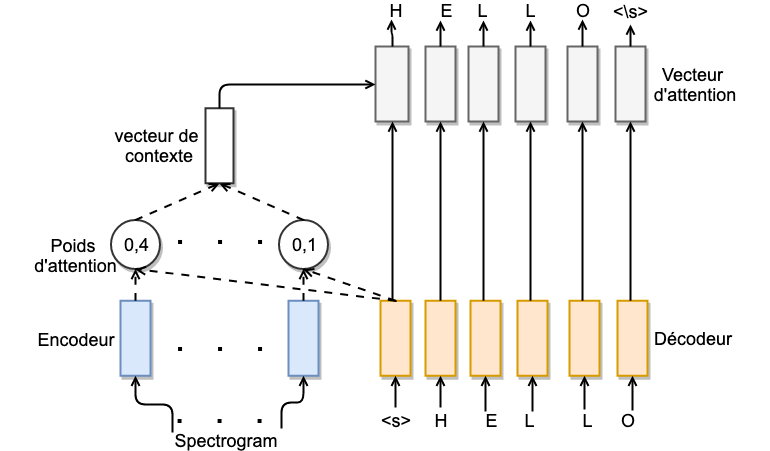
\includegraphics[height=205pt,width=365pt]{images/chap3/Att.png}
    \caption{Mécanisme d'attention}
    \label{atn}
\end{figure}

Nous pourrions introduire ce mécanisme en ajoutant une couche d'attention au modèle de base qui permettrait de relier les sorties de l'encodeur à celles du décodeur. Nous pensons que cette approche pourrait présenter un meilleur apprentissage. La figure \ref{archi_atn} schématise l'architecture d'un tel modèle.

\begin{figure}[H]
    \centering
    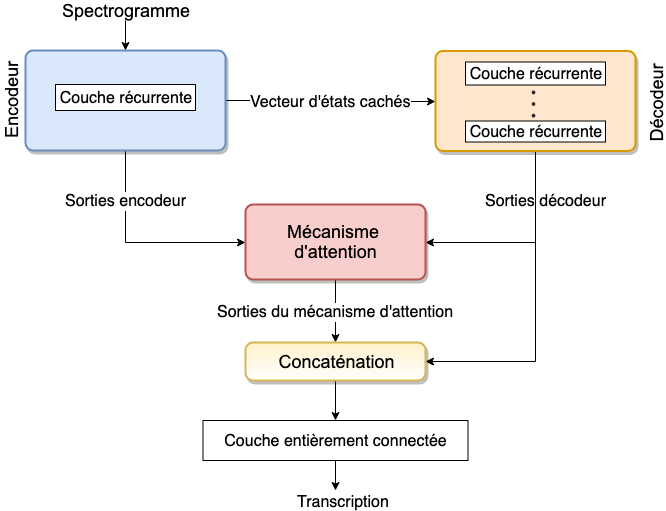
\includegraphics[width=320pt, height=240pt]{images/chap3/Attention.png}
    \caption{Architecture d'un modèle End-To-End avec mécanisme d'attention}
    \label{archi_atn}
\end{figure}

% Comme le montre la figure \ref{archi_atn}, le modèle de base se compose des modules suivants :
% \begin{itemize}
%     \item \textbf{Encodeur} : composé d'une couche récurrente et renvoie les vecteurs Hidden State mais aussi l'output de l'encodeur qui sera utilisé par la couche d'attention.
%     \item \textbf{Décodeur} : composé de plusieurs couches récurrentes où la première couche prend comme entrée les vecteurs Hidden State produits en sortie de l'encodeur.
%     \item \textbf{Mécanisme d'attention} : prend en entrée les sorties de l'encodeur et les sortie du décodeur pour effectuer un alignement des timesteps de l'entrée audio avec les timesteps de la transcription.
%     \item \textbf{Couche Fully Connected} : Dernière couche du modèle, prend en entrée l'output du décodeur.
% \end{itemize}

Pour clore, nous pouvons dire que la réalisation de ce projet nous a permis de maîtriser des domaines importants de l'intelligence artificielle. À travers ce travail nous avons : 
\begin{itemize}
    \item maîtrisé les principes de la reconnaissance automatique de la parole mais aussi les principes des systèmes de questions-réponses avec de potentielles applications très importantes que ce soit pour le web, applications mobiles ou autres plateformes, et
    \item approfondi nos connaissances en apprentissage automatique et maîtrisé de nouvelles approches plus flexibles et plus performantes nous permettant ainsi d'appréhender un grand éventail de problématiques d'intelligence artificielle. \\
\end{itemize}

En plus des compétences informatiques acquises, nous avons appris à gérer un projet, à rédiger un mémoire de qualité et à travailler en équipe tout en respectant les différentes conventions qui sont utilisées dans le monde professionnel. Au terme de ce projet, les enseignements s'avèrent être précieux et nous seront utiles tout au long de nos parcours respectifs.   
